\documentclass[11pt, headings=normal]{scrartcl}
\usepackage{spkb-pack}
\addbibresource{/Users/spkb/Documents/bibliographies/mybib.bib}






\usepackage{graphicx,grffile}
\makeatletter
\def\maxwidth{\ifdim\Gin@nat@width>\linewidth\linewidth\else\Gin@nat@width\fi}
\def\maxheight{\ifdim\Gin@nat@height>\textheight\textheight\else\Gin@nat@height\fi}
\makeatother
\setkeys{Gin}{width=\maxwidth,height=\maxheight,keepaspectratio}

\title{\bigskip \bigskip Japan's parochial press: Journalistic identity as structured weakness}
\author{\Large Scott Koga-Browes\vspace{0.05in} \\ \normalsize\emph{College of IR, Ritsumeikan Univ.} \\
\footnotesize \url{spkb@fc.ritsumei.ac.jp}\vspace*{0.2in}\newline
}
\date{\footnotesize 30 Oct 2017}

%%%%%%%BEGINNING OF DOCUMENT%%%%%%%
\begin{document}

\maketitle



\begin{abstract}
\noindent TBD
\end{abstract}

\hypertarget{introduction}{%
\section{Introduction}\label{introduction}}

Japan is home to a vigorous press, both national and local; levels of
newspaper readership have traditionally been high, and they remain so,
yet despite its apparently healthy state Japan's press is, in one sense
at least, in crisis; Japan has fallen down press freedom rankings over
the past few years. Particularly abrupt was the drop in its ranking
between 2010 and 2011/12 in the aftermath of the Fukushima Dai-ichi
nuclear disaster in March 2011. The situation for the press in Japan
seems to present two different faces; while the industry as a whole
seems to be healthier than many around the developed world, Japanese
journalism, and the journalists that produce it, is in a much less
confident mood.

\begin{figure}
\centering
\includegraphics[height=4.16667in]{./pix/rsf-fh-combined-with-comments.png}
\caption{\textbf{Figure 1:} Combined Reporters Sans Frontiéres
Press(RSF) Freedom rankings and Freedom House(FH) `Freedom of the Press
Score' for Japan, 2002-17. \label{fig:ranking}Sources:
\href{https://rsf.org/en/japan}{RSF},
\href{https://freedomhouse.org/report/freedom-press/2017/japan}{Freedom
House}}
\end{figure}

Japan's press still up there in the `free' zone but its ranking is at
the lowest level since the Reporters Sans Frontiéres(RSF) series began
in 2002, such a rapid fall - from 11th `free-est' in the world in 2010
to 72nd just six years later - must surely be cause for concern, at
least to the extent that a free press is a necessary part of a
functioning democracy. \Cref{fig:ranking} shows shows the decline in the
Japanese press' position in both Freedom House and RSF rankings; while
the RSF ranking is more volatile, they both show a continual fall in the
years after 2011. RSF noted that the precipitous drop after the 2011
triple disaster was in part due to complaints from freelance journalists
that `public debate was being stifled {[}\ldots{}{]} subjected to
censorship, police intimidation and judicial harassment.'\footnote{https://rsf.org/en/world-press-freedom-index-2013}

These concerns were further exacerbated during the debate over the
introduction of the `Specially Designated Secrets Protection Law' in
2013, which \textcite[1]{Repeta:2014} argues `poses a severe threat to
news reporting and press freedom in Japan'. In July 2015 the
International Press Institute's Director of Advocacy and Communications
Steven M. Ellis commented;

\begin{quote}
We are troubled that LDP members have engaged in acts that appear to
have placed improper political pressure on media
outlets{[}\ldots{}{]}Given the fundamental need for independent media in
a democracy, we urge Japan's leaders to ensure that media outlets'
ability to report freely is respected and to take steps to protect that
ability.\footnote{\href{https://ipi.media/pressure-on-japanese-media-raises-concerns/}{International
  Press Institute(IPI) Jul 2015}}
\end{quote}

Mounting concerned regarding the state of the press in Japan led to a
visit from the UN Special Rapporteur on the Promotion and Protection of
the Right to Freedom of Opinion and Expression, David Kaye, in October
2016. His visit confirmed the existence of a sense of unease within the
Japanese press, particularly with regards to its ability to maintain an
attitude of independence toward a government taking an increasingly
proactive approach to `press management'. During a press conference at
the end of his visit, Kaye summarised his experience of talking to
various actors within the Japanese mass media system as follows;

\begin{quote}
the problem is, the \textbf{system of journalism} and \textbf{the
structure of media itself in Japan} doesn't seem to afford journalists
the ability to push back against government encroachments, and you see
this {[}\ldots{}{]} in the example of the \emph{kisha} club\footnote{This
  paper uses the words `press club' as a translation of the Japanese
  term, \emph{kisha kurabu}. However it should be noted that the
  highest-profile `press club', the Japan National Press Club (in
  Japanese, \emph{Nihon Kisha Kurabu}), is entirely different from
  typical \emph{kisha kurabu} in its aims, membership and journalistic
  function.} system, we learned about serious concern about senior
members of the independent media meeting with senior members of the
government, we heard these stories repeatedly, and \textbf{I would
really encourage journalists to organise themselves, to adopt a
professional organisation, a union in effect, in which journalists can
express media-wide solidarity}, can perhaps enjoy self-regulation
through a press council, in short, the media itself has a role to play,
the media itself bears some responsibility for this situation (emphasis
added)
\end{quote}

He identified two particular tasks for those concerned with freedom of
the press in Japan: legal reform and `organisation'. This paper focusses
on `organisation' and looks at Japan's `system of journalism' and the
media structures that Kaye identifies as having a detrimental influence
on journalistic autonomy, and the difficulties which tend to block or
discourage professional-level organisation.

\hypertarget{background}{%
\subsection{Background}\label{background}}

Japan must be understood as a (in this case genuine) special case: The
mainstream media in Japan is highly dominant in a very isolated market,
Japanese readers, unlike (for example) readers of English in the UK, do
not have the luxury of turning to say the US, Australian or even Russian
press for alternative views. Japanese media firms are virtually the only
producers of Japanese-language news and information.\footnote{Some
  exceptions - such as news sites catering for Japanese overseas
  communities in Asia and the Americas, e.g.
  {[}http://www.nikkeyshimbun.jp/{]}. The 海外日系新聞放送協会 OJPA
  claims 20 members, the majority of whom are based in South
  America.\href{http://www.jadesas.or.jp/shinbun/}{OJPA} - 4 Jan 2017.}
The seven \emph{zenkokushi} (newspapers with national daily
reach\footnote{This report does not identify which newspapers it
  considers \emph{zenkokushi}; these are probably the five main national
  dailies mentioned previously plus \emph{Akahata}, produced by the
  Japan Communist Party, \emph{Seikyō Shimbun}, produced by the
  religious group Sōka Gakkai, or the English-language \emph{Japan
  Times}.}) employ just under 20,000 staff, about half of these in
editorial roles\footnote{\href{http://www.meti.go.jp/statistics/tyo/tokusabizi/result-2/h27.html}{Ministry
  of Economy, Trade and Industry (METI) Special Service Business Report
  2015}}. Between them they have daily sales of roughly 30 million
copies, that is they supply daily news to over half of Japan's 52
million households.\footnote{http://www.stat.go.jp/english/data/nenkan/66nenkan/index.htm}
Add to this the influence of the main news agencies, Kyodo News
(\href{http://www.kyodonews.jp/english/}{Kyōdo Tsūshin-sha}) and Jiji
Press (\href{http://jen.jiji.com/}{Jiji Tsūshin}), who supply news to
newspapers, and radio and television broadcasters\autocite[59]{JMH:2015}
(CITATION! RAUSCH? \autocite{Rausch:2012}), it can be seen that there is
little scope for alternative, `left-field' or even `non-mainstream'
voices.\footnote{the repeated failed attempts at `public journalism'
  (see, for example, \textcite{ItoT:2005}) and the mobilisation of the
  `citizen reporter' (see
  \href{http://www.nytimes.com/2010/06/21/world/asia/21japan.html}{Fackler})
  also seems to point to this dominance, and also perhaps a lack of
  interest on the part of audiences for `alternative' sources.
  MyNewsJapan etc.} Kyodo claim over 170\footnote{http://www.kyodonews.jp/company/members.html}
national outlets as clients, Jiji another 140\footnote{http://www.jiji.com/c\_profile/about\_us.html}.

It should also be noted that the possibilities for alternative
journalistic forms that have arisen with the spread of the internet have
not affected the mainstream media in Japan as they have many other media
systems around the world. In 2010 Martin Fackler, the \emph{New York
Times'} Tokyo correspondent wrote:`No online journalism of any kind has
yet posed a significant challenge to Japan's monolithic but sclerotic
news media'\autocite{Fackler:2010}.\footnote{http://www.nytimes.com/2010/06/21/world/asia/21japan.html}
His assessment is born out by the fact that web-native,
citizen-journalist and participatory news services such as
JanJan(2002-2010), PJNews(2005-2012) and OhmyNews Japan(2006-2008) ---
despite the enthusiasm and hopes for their transformative role in
Japan's media environment that accompanied their springing up in the
early to mid '00s \autocite[ 72--3]{Hadl:2009} --- have not lasted in
Japan. Thus the structures that shape the way the \emph{mainstream}
media report events, and in which the mainstream press is particularly
implicated, matter perhaps more deeply in Japan than in many other
modern industrial states.

As far as broadcast news is concerned, the picture is similar; the most
watched news program, the \emph{Nihon Hōsō Kyōkai} (NHK) early evening
news programme (\emph{Nyūsu 7}) is regularly watched by 16-17 million
people, news on commercial channels brings in combined audiences of over
30 million; the top-rated commercial news shows, TV Asahi's \emph{Hōdō
Station} and NTV's early evening \emph{news every} regularly have 12--14
million viewers.\footnote{This adopts the rough approximation, 1 per
  cent = 1 million viewers, suggested by \textcite[29]{Torigoe:2002}.
  This estimate is close to the estimate offered by Ozeki Kōji,
  torishimariyaku at Video Research in an interview with TV Asahi
  (\emph{Hai! Terebi Asahi desu}) broadcast on 19 Feb 2017. Figures
  compiled from Autumn 2016 ratings data -
  \href{https://www.videor.co.jp/data/ratedata/backnum/2016/index.htm}{Video
  Research}} These are all national programs and the only local
programming to gain similar ratings is that produced by NHK for the
Greater Tokyo region (\emph{shutōken}), home to just under a third of
Japan's population.

It should be noted that it is these major media companies --- six
Tokyo-based television networks, the five major national daily
newspapers, and the two national news agencies --- that make up the core
13 members\footnote{Broadcasters: NHK, TV Asahi, Nippon TV, Fuji TV,
  Tokyo Broadcasting Systems(TBS) and TV Tokyo. Newspapers: Yomiuri
  Shimbun, Asahi Shimbun, Mainichi Shimbun, Sankei Shimbun and Nihon
  Keizai Shimbun (Nikkei). News agencies: Jiji Tsūshin and Kyōdō
  Tsūshin.} of many of the `press clubs'.

\hypertarget{aims}{%
\subsection{Aims}\label{aims}}

Ultimately the question this paper seeks to address is: Why, given the
obvious concern with independence and what Kaye describes as the deep
commitment to freedom of speech and expression in Japan, and the obvious
concern of many journalists, have news-workers in Japan not organised in
the way he suggests?

{Also review bodies in Japan for reporters and those involved in news.
Brief review of reporting organisations.}

REMEMBER: \textbf{`systems' and `structures'} {TODO}

This paper argues that the root causes of this failure to organise, can
be found in a) the nature of the professional education of journalists,
and b) the nature of employment structures for journalists in Japan. The
effects of these social institutions can be observed manifested as the
`professional ideology' of journalists in Japan, this paper uses certain
aspects of this ideology as proposed by \textcite{Deuze:2005}.

This has led to a situation where reporter identity is centred on
entities - companies as employers - which are required (at least as far
as rhetoric is concerned) to be in a relationship of `fierce
competition'.

Are Japanese journalists equipped to push back against the forces that
pressure them? Can the `professional identity' of the journalist be seen
as a protective barrier, a layer of insulation, which allows journalists
a psychological cushion and promotes the kind of activity and
relationships expected of the ethical journalist. Does the lack of this
cushion contribute to the state of journalism in Japan at the current
time?

This paper will not deal with the influence if the \emph{kisha kurabu}
`press club' system, probably the most widely documented aspect of
journalism in Japan, as it has been dealt with extensively elsewhere
\autocites[see for
example][]{Lange:1998}{Freeman:2000}{Iwase:1998}{Yamamoto:1989}, but it
is worth summarising the effects of press club journalism; the
collective responsibility implied by press club membership leaves the
press open to pressure both from peers - to not rock the boat and upset
relations with sources - and from sources who can deny access more or
less at will. Given the possibilities offered by social media for
politicians to simply bypass the mainstream media, it is difficult to
see how the traditional `balance of power' for control of access (press
to politicians, politicians to the public) can be maintained. Japanese
politics has been rather late to the social media jamboree with the use
of online campaigning in general elections prohibited until 2013, but
this will change \autocite[p51]{Osaka:2014}.

\hypertarget{systems-and-structures}{%
\subsection{Systems and Structures}\label{systems-and-structures}}

Journalism may well be best ultimately described in terms of a set of
norms, ideas and beliefs that might adequately be characterised with the
term ideology \autocite[for example, see][]{Deuze:2005}. The exact
contents and structures of this ideology will vary across systems and
across periods; this paper looks rather at the structures and groups
within which this set of ideology is learned, the process of
identification through which it becomes internalised by the individual
journalist. Specifically it looks at the structures and systems
identified by Kaye (see above) as being inimical to the Japanese
journalist's ability to push back against political pressure.

Discussion of the elements of the nature of the journalistic identity
has been an integral part of academic understandings of news and
news-gatherers since the very early days of the field (eg?).
Deuze\autocite*{Deuze:2005} sums up the essential features of what he
refers to as the journalistic ideology as `public service',
`objectivity', `autonomy' and a sense of both `immediacy' and
`ethics'\autocite[p447]{Deuze:2005}. Where and when are the norms,
values and beliefs about journalism acquired?

Some of Minami's interviewees point toward their experiences of formal
education as a fundamental site for the acquisition of their
understanding:

\begin{quote}
those who have a degree in journalism say they learned what journalists
should be through journalism education in college
\autocite[214]{Minami:2011}
\end{quote}

\emph{ANSWER THIS FOR THE GENERAL CASE}

What has been the effect of a strong bureaucratic tradition on the role
of professional ideas in journalism in Japan?

`Sectionalism' (Shimizu?) \emph{Tate-wari}

\hypertarget{journalism-in-japan}{%
\section{Journalism in Japan}\label{journalism-in-japan}}

{LIT REVIEW in here}

Japan has a history of journalism stretching back to its emergence from
under the control of the Tokugawa Bakufu in the latter decades of the
nineteenth century. Early journalism was often politically sponsored and
overtly partial, the individuals considered japan's first modern
journalists --- Yanagawa Shunsan\footnote{Japanese names are given in
  traditional surname-first order except where the individual is well
  known by the surname-last version.} (1832-70) publisher of the
\emph{Chūgai Shimbun}, and Fukuchi Gen'ichiro, well known for his work
at the \emph{Tōkyō Nichinichi Shimbun}\autocite[32]{Huffman:1997} ---
had `close personal ties to the \emph{bakukfu} shogunate'
\autocite[p9]{Schafer:2012}.

Japan's press in many ways reproduced similar changes, those driven by
the growth of cities and changes in printing and distribution
technologies, that had happened in other developed countries around the
world \autocite[see, for example][3--4]{McChesney:2003a}; it was as the
twentieth century entered its second and third decades that, with the
adoption of the `objective' mass circulation model and the production
techniques that made them possible, that the press began to require
something like the `professional' journalist --- an objective, detached
observer --- rather than the partisan supporter and advocate. The trauma
and reconstruction of pre- and postwar decades

\textcite[12--3]{Shibata:2003} suggests that the current worrying state
of journalism in Japan began to take place in the aftermath of the
Vietnam War; during this period newspapers in Japan had maintained an
`opposition party spirit' (\emph{yatō seishin}) and had been critical of
both US and Japanese foreign policy in Southeast Asia. From the mid-`70s
the \emph{Sankei Shimbun} broke ranks and began to take a more
government (Liberal Democratic Party / \emph{Jimintō}) friendly line, it
was followed in the '80s by the \emph{Yomiuri} with its
pro-Reagan/Nakasone stance. This led to the current situation with the
\emph{Asahi} and \emph{Mainichi} on the oppositional side and the
\emph{Yomiuri} and \emph{Sankei} being conservative,
pro-(LDP)government. As Shibata states, it is perfectly reasonable, and
indeed desirable, for newspapers to offer different point of view to
their readers, but, he argues, the shifts in the attitudes of two of
Japan's largest papers fundamentally affected the ability of the press
to perform their 'watchdog' function.{QUOTE better?}

\hypertarget{development-of-journalism-as-a-trade}{%
\subsection{Development of journalism as a
trade}\label{development-of-journalism-as-a-trade}}

The first move to give form to journalism as a trade in Japan was the
\autocite[10]{Schafer:2012} 1875 formation of the Alliance of Newspaper
Reporters (\emph{Shimbun Kisha Rengō}) in reaction to increasingly
restrictive laws which affected the press and protection against
libel.\footnote{\emph{shimbunshi jōrei}, \emph{zanbōritsu}}

Graduates of Japan's first universities, the University of Tokyo (1877)
and Waseda (1882) began to move into journalism during the 1880s and the
number of graduate journalists has gradually increased since. During the
1920s, economic recession meant a dearth of graduate employment
opportunities at a time when the popular press was expanding and looking
to increase the quality if its content by employing better educated
reporters.\autocite[36]{Schafer:2012}

During the years of political turbulence between the 1880s and the first
decade of the 20th century, the nature of the relationship between
politics and the press underwent a series of changes involving
adjustments of the relationships between newspapers, politics and an
expanding `public'. \textcite{Kawabe:1921} relates his view of these
changes from a vantage point at the start of the 1920s; one recurring
theme in his narrative of these changes is the way that journalists in
these years acted together to oppose policies they thought acted against
their interests, or impede their ability to carry out their work, and
thus, to keep their publics informed. It seems that the now
much-criticised `press clubs' were, during this period, a focus for
journalistic action. \autocite[see especially][155--9]{Kawabe:1921}

The \emph{Shimbun Kisha Kyōkai} established in Tokyo in December 1920
seems to have been primarily conceived of as a way of putting pressure
on employers to improve working conditions and pay. This organisation's
attempt to contribute to the status of reporters by introducing a
examined qualification\footnote{called the \emph{shimbun-shi} (新聞士),
  synonymous with the \emph{gakushi} (学士), or `bachelor's degree'. See
  \textcite[122-133]{Kawasaki:2006} for details.} based on a similar
proposal made by ex-reporter and Illinois Lieutenant Governor Barratt
O'Hara, was rejected by the majority of working reporters, primarily on
the basis of doubts over whether the skills necessary for reporting
could be meaningfully `examined' and whether any such qualification
would actually lead to any improvement in the quality of journalism. On
the other hand, voices raised in favour saw it as a way of heading off
government interference.\autocite[124--5]{Kawasaki:2006}

However along with this shift toward employing individuals who had
passed through the system of imperial universities - and reducing the
number of `enthusiasts' - who saw themselves as `educators of society' -
came an increase in the number of `company employees'. In 1917, Motoyama
Hikoichi\footnote{journo at \emph{Osaka Shinpō}, then \emph{Jiji
  Shinpō}, 1888 reorganised \emph{Osaka Mainichi SB}, became pres in
  1903: Advocate of foundation of newspaper studies depts at univs and
  later president of \emph{Osaka Mainichi} newspaper
  \autocite[36n]{Schafer:2012}.} had characterised this shift with the
following words,

\begin{quote}
a journalist, just like a salaryman of any other profit-oriented
company, needs to spare no efforts in favor of his company.
\autocite[37]{Schafer:2012} citing \autocite[52]{Ono:1971}
\end{quote}

The journalist was increasingly seen as primarily a company employee
like any other. And the \emph{shimbun-gaku} `newspaper studies'
departments established at universities were aimed at providing
potential journalists with the requisite knowledge to allow them to gain
employment at newspapers on graduation. It took until 1929 for a Tokyo
Imperial University to establish a `Newspaper Research Seminar' as part
of its literature department.\autocite[ p40]{Schafer:2012}

Ono Hideo was the prime motivator in the establishment of this body, he
saw the professional training he sought to offer as a way to push back
against the `degeneration' of the press he perceived in the 1920s, and
to raise journalists who would again act as educators of society,
ensuring that expert and specialist opinion would be made available to
the newspaper's mass audience \autocite[ p45--5]{Schafer:2012}.

It can be seen that discussion of the role of formal journalistic
education has not been lacking in Japan; nevertheless, despite what
seems to be an acknowledged consensus on the part of educators that such
an education would be beneficial (they would say that wouldn't they) few
Japanese tertiary institutions offer any sort of practical journalism,
probably due to the lack of enthusiasm on the part of potential
employers who continue to place little value on specialist knowledge.

\autocites{Huffman:1997}{Lange:1998}

\hypertarget{education-of-journalists}{%
\subsection{Education of Journalists}\label{education-of-journalists}}

Deuze, in his typology of global journalism education approaches,
categorises the Japanese system as characterised by

\begin{quote}
{[}p{]}rimarily on-the-job training by the media industry, for example
through apprenticeship systems (Austria, Japan; Great Britain and
Australia started this way, as this is a typical feature of the
Anglo-Saxon model).\autocite[ p22]{Deuze:2006}
\end{quote}

It should be noted that the US is not included in the `Anglo-Saxon'
model, instead being grouped with countries which prefer:

\begin{quote}
{[}t{]}{]}raining at schools and institutes generally located at
universities (see e.g.~Finland, Spain, United States, Canada, South
Korea, Egypt, Kenya, Argentina, the Gulf States, increasingly in Great
Britain and Australia \ldots{})
\end{quote}

It should be noted that the Japanese press' attitude towards its work,
and its wider role within society, and indeed some its it fundamental
regulatory structures (see BROADCAST LAW), is based on the `objective'
model established in the US in the early part of the 20th century, yet
the way it educates and trains its journalists is still close to the
systems which emerged in the highly politicised and openly partial press
found in the UK and Australia. {REFME}

See parts of\ldots{}

\autocites{Cooper-Chen:1997a}{Fujita:2004}{Hanada:2003}{Hashimoto:2003a}{Ikuta:2004}{IwabuchiY:2004}{Tsukamoto:1993}{Tsukamoto:2006}

Also refer to \textcite{Aldridge:2003}.

Employer indifference to journalistic education has been a continuing
feature of the Japanese system since at least the immediate
post-Occupation period:

\begin{quote}
There was a pressing need for journalism education after the war. But
this does not necessarily mean that students with training in journalism
are assured of employment after graduation from college. In the first
place, education in journalism is not appreciated by newspaper
publishers as an asset to reporters. It is true that most of the daily
newspaper in the country employ only college graduates but their
publishers still hold \ldots{} `The only place one can learn to be a
journalist is in a good newspaper office.' They want to train their cub
reporters in their own shops to their own liking. Hence college
graduates could not expect to draw any advantage out of their
professional training when they go out of school. \autocite[
326]{Chiba:1952}
\end{quote}

Indeed, outside employment there is little opportunity for potential
journalists in Japan to acquire knowledge, skills and experience of
their chosen trade. \textcite[135]{Splichal:1994} surveyed students in
journalistic education in 22 countries in the mid 1990s, they found that
90 per cent of Japanese respondents had no experience of engaging in any
sort of journalism before entering their course, the highest proportion
of any of the countries surveyed. The average rate for all countries was
just over 60 per cent.

As a route to employment an education in journalism can be all but
irrelevant, as \textcite[22]{Cooper-Chen:1997a} suggest, company
recruitment relies on testing general skills (general knowledge,
literacy) so a degree from \emph{any} department in a prestigious
university may be worth more than specialist knowledge from a less
prestigious institution. Theses attitudes and the expectations of media
employers - virtually no value attached to any sort of university-based
journalistic education \autocite[1]{Fujita:2004} in Japan seems to go
back to at least the 1930s \autocite[14]{Uchikawa:2003}.

\textcite[167]{Willnat:2013} found that over 95 per cent of journalists
in Japan had a college degree, among the highest rate of countries
surveyed, yet the proportion of those with a degree specifically in
journalism was the second lowest at just 15 per cent. Japan also had the
oldest average age for journalists at 53, seeming to indicate that,
unlike many other countries, journalists in Japan tend to stay in their
work longer. An overwhelming majority of Japanese journalists surveyed
for this work recognised training as an area requiring
improvement:`(82.9\%) noted that there is a clear need to improve
journalism education and training in Japan' \autocite[ 62]{Oi:2012}.

\textcite{Fujita:2004} points to changes in the environment as a cause
of the growing perception that the `on-the-job training' (OJT) system
was not producing the desired results, this led to a renewed debate
about the role of university-based journalist education in Japan in the
later 1990s and early '00s - the increasing use of technology at all
levels of newspaper production and the increased pressure on workers
which left little time for senior reporters to train new
staffers.\autocite[3]{Fujita:2004}

This debate took place in reaction to a number of incidents
(plagiarism\footnote{About one-third of an article in the 8 Jun 2000
  edition on the \emph{Asahi Shimbun} was found to have been plagiarised
  from the local \emph{Chugoku Shimbun} by a reporter in the Hiroshima
  office.\autocite[137]{Shibata:2003}}, invasions of privacy,
`overheated' herd reporting (\emph{media sukuramu}),
libel)\autocite[1]{Ikuta:2004}. Ikuta also identifies the pressures of
adapting to new technologies as a root cause in the drop in journalistic
standards.

Ikuta describes the actual content of OJT at the \emph{Asahi Shimbun};
new employs spend four or five years at a local office where their
development can be overseen trained by experienced reporters,
traditionally the local office would be a mix of new, middle career and
`veteran' reporters. However Ikuta argues that this system broke down
due to the HR policy of concentrating middle-career reporters in the
head offices, which led to an over-reliance on early-career reporters in
local bureaus. (ibid. p224/1180) This breakdown seems to be confirmed by
one of the junior journalists interview by \textcite[242]{Minami:2011},
`Shota' explains;

\begin{quote}
In the past, editors or managers would take care of young reporters in
their departments. They had time and room to do that. They used to take
young reporters out for drinks or something after work. But nowadays,
their workload has also increased so that they have lost such leeway.
So, they can't pay close attention to what young reporters are doing.
It's kind of a vicious cycle.
\end{quote}

A significant effect of a primarily OJT-based system might be that it
becomes more difficult to have any external standard (what kind of
standard?); if the measure of professionalism is how closely one
approximates the work of one's mentor then it is easy for
\emph{practical} understandings of how one does journalism --- rather,
how one does the job of journalist --- to become prioritised over how
should (according to some exterior abstract measure - whether a code, an
exemplar or whatever) journalists set about doing their work. It might
also be readily supposed that such a system might turn out to be more
`malleable' from the political sources' point of view with the local (in
time and space) understandings of the necessities of practical reporting
being passed on, and thereby taking on the status of `common sense',
within a single generation.

\hypertarget{sources-of-ethics}{%
\subsection{Sources of Ethics}\label{sources-of-ethics}}

A shared understanding of what it is that a journalist does, and what
separates those who can justify a claim to be journalists from those
whose claims can be refuted, is linked to the possibility of claiming to
be acting in accordance with an understood set of ethical rules,
specifically one formulated by a recognised arbiter of journalistic
activity.

\begin{quote}
Both the creation of codes of ethics and the emergence of formal
education and training for journalists fostered a shared culture among
journalists. \autocite[ 66]{Tumber:2005}
\end{quote}

What are the sources of ethical understandings in Japan? How widely are
these shared across groupings within the industries in which journalism
takes place? Section below covers this (see
\protect\hyperlink{ethics}{below})

\hypertarget{journalistic-employment-in-japan}{%
\subsection{Journalistic Employment in
Japan}\label{journalistic-employment-in-japan}}

The The Japan Newspaper Publishers and Editors Association
(NSK-JNPEA\footnote{This body also refers to itself by the acronym NSK,
  formed from the initial letters of its Japanese language name, the
  \emph{Nihon Shinbun Kyokai}, literally, Japan Newspaper Association.
  \href{http://www.pressnet.or.jp/english/}{JNPEA/NSK website} This
  paper uses NSK-JNPEA throughout.}) carries out annual surveys of
employment within the newspaper industry; according to these surveys
there are approximately 20,000 `reporters', this number has remained
more or less constant over the past 15 years (see figure N). In the same
period the total number of newspaper employees has dropped from 54,565
in 2001 to 41,396 in 2016. The proportion of employees engaged in
reporting work has thus increased from 38 per cent of the total
newspaper workforce in 2001 to 46 per cent in 2016.\footnote{http://www.pressnet.or.jp/data/employment/employment03.php}

\begin{figure}
\centering
\includegraphics[height=4.16667in]{/Users/spkb/pix/j-employees.png}
\caption{Change in employee numbers in the Japanese newspaper industry;
percentage change taking 2001 as index value. Source
\href{http://www.pressnet.or.jp/data/employment/employment02.php}{NSK
Website}}
\end{figure}

A government survey from 2016 counts 7 national dailies, 245 regional
and local papers, and 4 `sports' papers, as well as 514 specialist and
industry journals. The national, regional/local and `sports' press in
total employ 44,331 people, 9508 women. Just over a fifth of the
newspaper workforce is female. 36,293 are full-time employees
(\emph{sei-shain}), this includes 6044 (apx.17\% of total) female
workers. Newspaper work is an overwhelmingly male undertaking.

For purposes of comparison, the US newspaper industry in 2001 employed
411,800 people, this figure had fallen to 174,709 by September 2016.
(Source: US Bureau of Labour \footnote{https://www.bls.gov/opub/ted/2017/newspaper-publishers-lose-over-half-their-employment-from-january-2001-to-september-2016.htm})

What are their backgrounds? Who are they?

See \textcite{Kawasaki:2006} for historical background. {TODO}

Average career length?

Typical career development?

Careers develop largely within a single company, or companies and
organisations within the same group, or `somehow' affiliated. E.g.
senior editorial staff may, towards the end of their working lives, find
themselves in senior positions on the boards of local television
broadcasters.

{check interlocking boards?}

\textcite{Minami:2011}

\emph{Tenshoku}?

Chiba Yūjiro, a reporter for the \emph{Asahi Shimbun} during the 1930s
and later a senior academic working at the Newspaper Research Institute
at Tokyo University, writing at the end of the US occupation in 1952,
pointed to the relationship between employment structures and the
development of a shared professional - in the sense of paid employment -
identity:

\begin{quote}
In the second place, lack of solidarity on the profession operates as a
barrier to the transfer of journalists from a local newspaper to a
metropolitan newspaper, where openings are limited. \autocite[
326]{Chiba:1952}
\end{quote}

\hypertarget{press-clubs}{%
\subsection{Press Clubs}\label{press-clubs}}

The role of the `press club' (\emph{kisha kurabu}) shoudl also be
mentioned as this where much journalistic activity takes place and is a
primary site for interactions between journalists across company lines,
that is \emph{as journalists rather than as employees}.

Press clubs, while much vilified (rightly so), are a situation where
cooperation, of certain types, between journalists is taken for granted.
Indeed in the past these clubs have acted as a focus for journalistic
solidarity crossing company lines:

\begin{quote}
By about 1930, the clubs themselves had expanded enormously and had
begun to act independently of the newspaper companies. Sometimes, when a
financially troubled newspaper would try to reduce its staff or a paper
would try to fire an incompetent reporter, the club as a whole -
including, of course, reporters from other newspapers - would rise up to
demand that its member be rehired. \autocite[ 386]{Yamamoto:1989}
\end{quote}

The newspaper industry and journalistic work were, in the 1930s, far
less professionalised and the landscape of media companies was in the
process of development and less ossified than it is today. In this
sense, given the power of the company today, it may be difficult for the
press club to recapture its role as a site of cross-firm cooperation.
However, it would be unwise to entirely overlook them as a possible site
for expanded types of cooperation.

Realistically, skeptically perhaps, it is easier to see the \emph{kisha
kurabu} as yet another fracturing element of journalistic identity:
\textcite[70--1]{Freeman:2000} lists the various \emph{kisha kurabu}
attached to central government agencies and ministries in Tokyo, the
majority of them are host to more than once club, the Ministry of
Transportation and the Ministry for International Trade and Industry
both have seven different clubs listed for them.

\hypertarget{sources-of-autonomy}{%
\section{Sources of Autonomy}\label{sources-of-autonomy}}

This concept at the core of the argument presented in this paper.

What is it that allows the journalist this autonomy? Identity as a
professional that extends beyond the fact that they work for a company
which `does news'. Basis for maintaining the `chinese wall' between
business and editorial, insulation from source pressure etc.

The Japanese journalist, as a result of the diversity of educational
backgrounds - surely a strength in terms of diversity of knowledge -
lack a strong external power base \autocite[212--3]{Soloski:1989}

To be autonomous invites suspicion - to be outside a publicly
legitimised organisation - the reputation of trades unions, other than
the `company unions' prevalent across much of Japanese industry is as
`trouble makers obsessed with Marxist doctrine'(CHECK!) - is to lose a
credibility and social trust. Thus, without some sort of legitimate (by
whose standards?) body to which they can refer, journalists are
effectively restricted to acting within the bounds of the vertical
company-based structure. The `media-wide' cooperation that David Kaye
referred to necessary to effect a concerted push back against top-down
pressure is near impossible.

\begin{quote}
ジャーナリストというより朝日新聞社員としての仕事をしている図式です
\end{quote}

quote from - 新聞協会賞を2度受賞した\emph{依光隆明}朝日新聞社編集委員
\autocite{JCEJ:2014}

Then there is the question of industry autonomy from government power.
The structures of the mass media (and in the broader economy in which
media companies exist), gradually put in place over the 70 years since
the end of WW2, has turned out to be a double-edged sword. The sections
below focus on the linkages between legislation/regulation and media
industries which can be seen as political pressure points, which are
none the less so for not being employed as such.

\hypertarget{the-broadcast-act}{%
\subsubsection*{The Broadcast Act}\label{the-broadcast-act}}
\addcontentsline{toc}{subsubsection}{The Broadcast Act}

Identified by Kaye as an obvious political pressure point. Takaichi
Sanae statements during 2015/6.

Kaye suggests some third party regulator equivalent to the US Federal
Communications Commission(FCC). Such a body, the Radio Regulatory
Commission (RRC), did exist for just over one year during the period
between the passing of the Broadcast Act and the end of the US
occupation; the body's two most significant acts were to grant a
broadcast licence to Japan's first commercial broadcaster, Nippon TV,
and then to dissolve itself, returning control of broadcasting to a
ministry (at that time the Ministry of Posts,
\emph{Yūsei-shō}).\autocite[41]{Ito:2010} So, while there is a precedent
for such a body, it is not an altogether promising one.

What are the problems with the Broadcast Act?

Article four is divided into two sections, the first deals with
programming content, the second with encouraging broadcasters to provide
services for the visually impaired. It is the first section (see below)
which Kaye refers to.

\begin{quote}
\textbf{Article 4}

(Editing and Other Matters of the Broadcast Programs of Domestic
Broadcasting, etc.)

The broadcaster shall comply with the matters provided for in the
following items when editing the broadcast programs of domestic
broadcasting or domestic and international broadcasting (hereinafter
referred to as ``domestic broadcasting, etc.''):\\
(i) It shall not harm public safety or good morals;\\
(ii) It shall be politically fair.\\
(iii) Its reporting shall not distort the facts;\\
(iv) It shall clarify the points at issue from as many angles as
possible where there are conflicting opinions concerning an issue.
\end{quote}

The other article with direct relevance to the current debate is article
174 which holds out (for some at least) the possibility of governmental
action to sanction broadcasters.

\begin{quote}
\textbf{Article 174}

(Suspension of Operations)

If the broadcaster (excluding terrestrial basic broadcasters) has
violated this Act or an order or disposition based on this Act, the
\textbf{Minister of Internal Affairs and Communications shall set a
period within three months and shall order the suspension of the
operations of the broadcasting}. (emphasis added)
\end{quote}

According to arguments put forward in \emph{Hōsō Repōto} the government
may not actually be justified in using the Broadcast Act in this way
\autocites{Hara:2016}{Hara:2017}. Any interpretation of the relevant
articles which sees them as a basis for regulatory interference on the
part of government undermines the basic tenets of the Broadcast Law
which assures that broadcasting should be `free and independent'
(\emph{hōsō no jiyū to jiritsu}) \autocite[3]{Matsuda:2016}

Indeed in submissions to a committee looking at broadcast related laws
in 1964\footnote{\emph{Rinji Hōsō Kankei Hōsei Chōsa-kai} (see
  \textcite{Hara:2017}, 56)}, bureucrats from the Ministry of Posts and
Telecommunication (\emph{Yūsei-sho}, MPT) stated that:

\begin{quote}
\ldots{} in practical terms, these are `goals to be aimed for', as for
the actual effects of the law, {[}we{]} consider that they go no further
than being moral guidelines (\emph{seishinteki kitei}) (author's
translation)
\end{quote}

This stance was repeated by senior ministry bureaucrat, Ishikawa Teruo?
in responses to a Diet Upper House Committee question on 27 April 1977.
The interpretation changed some time in the mid-1980s in response to
what was seen as an increasingly overt licentiousness in overnight
commercial programming, and perhaps triggered by the broadcast on TV
Asahi's \emph{Afutanūn Shō} (Afternoon Show) of (what turned out to be)
a fake news story about the lynching of a junior high-school girl. From
this point on regulators at the MPT were to repeatedly state that - in
contrast with what had been the position previously - Article 4 of the
Broadcast Law could now be taken taken to offer a basis for regulatory
sanctions, \emph{gyōsei shidō} (administrative guidance), of the sort
common in Japanese governance, for example the issuing of \emph{keikoku}
(`warning') or \emph{genjū-chūi} (`strict
caution') \autocite[57]{Hara:2017} However, what seems to have
broadcasters concerned is not necessarily this gradual re-interpretation
of the Broadcast Law but the apparent shift, signalled by Takaichi Sanae
in 2015, in the scope of its possible applicability. Rather then
broadcasters being sanctioned for repeated `violations', that is, the
failure to self-regulate efficiently and promptly, Takaichi raised the
possibility of regulatory sanction for \emph{individual programs} which
in the opinion of government failed to meet the standards of Article 4.
\autocite[57]{Hara:2017}

\hypertarget{newspaper-sales}{%
\subsubsection*{Newspaper Sales}\label{newspaper-sales}}
\addcontentsline{toc}{subsubsection}{Newspaper Sales}

\begin{itemize}
\tightlist
\item
  Weakness of JFTC
\item
  Pricing cartel
\item
  \emph{Saihan seido}
\end{itemize}

The \emph{tokushū shitei} status of newspapers is a purely regulatory
matter, the JFTC could decide to rescind it at any point. Occasional
government reassessments of its social value serve to remind the
newspaper industry of this.

\hypertarget{ethics}{%
\subsection{Ethics}\label{ethics}}

Also see Society of Professional Journalists Ethics Guide.\footnote{https://www.spj.org/ethicscode.asp}

\hypertarget{the-nsk-ethics-guide}{%
\subsubsection{The NSK-JNPEA Ethics Guide}\label{the-nsk-ethics-guide}}

The NSK-JNPEA is one source of guidance on journalistic ethics\footnote{新聞倫理綱領\\
  2000(平成12)年6月21日制定\\
   21世紀を迎え、日本新聞協会の加盟社はあらためて新聞の使命を認識し、豊かで平和な未来のために力を尽くすことを誓い、新しい倫理綱領を定める。\\
   国民の「知る権利」は民主主義社会をささえる普遍の原理である。この権利は、言論・表現の自由のもと、高い倫理意識を備え、あらゆる権力から独立したメディアが存在して初めて保障される。新聞はそれにもっともふさわしい担い手であり続けたい。The
  citizen's right to know is the unshakeable principle upon which the
  democratic society is built. It is only with a media independent of
  all power and equipped with a string sense of ethics based in the
  freedoms of debate and expression, that this right is guaranteed.
  {[}We desire that{]} newspapers continue to be the most suitable means
  for this.\\
   おびただしい量の情報が飛びかう社会では、なにが真実か、どれを選ぶべきか、的確で迅速な判断が強く求められている。新聞の責務は、正確で公正な記事と責任ある論評によってこうした要望にこたえ、公共的、文化的使命を果たすことである。{[}\ldots{}{]}
  The duty of the newspaper is to respond to the desire {[}for speedy
  and accurate decisions in choosing truth from the welter of
  information now available{]} to carry out its public and cultural
  mission.\\
   編集、制作、広告、販売などすべての新聞人は、その責務をまっとうするため、また読者との信頼関係をゆるぎないものにするため、言論・表現の自由を守り抜くと同時に、自らを厳しく律し、品格を重んじなければならない。All
  newspaper workers - editorial, production and advertising - to fully
  perform this duty, and in order to ensure that an unshakeable bond of
  trust with readers, at the same time as ensuring they safeguard
  freedom and speech and expression, must maintain a strict self-control
  and value dignity (of what?)}, its Canon of Journalism\footnote{\href{http://www.pressnet.or.jp/outline/ethics/index.html}{Canons}}
was most recently updated in June 2000. When compared to similar sets of
guidelines provided by organisations in other countries, numerous
differences are immediately apparent. The NSK-JNPEA guide offers little
in the way of practical advice for journalists it's articles consisting
primarily of high-flown exhortations to, for example, `put a high value
on individuals' honor and give serious consideration to their right to
privacy' - what this might entail in practice for the journalist going
about their everyday work is not outlined. More important for the topic
of this paper, it should also be noted that the \emph{subject} of the
NSK-JNPEA code is more often `the newspaper'(\emph{Shimbun}), `the
member company'(\emph{kamei-sha}) rather than the individual journalist,
the term for journalist or reporter (\emph{kisha}) appears only twice.
This again would seem to point to the central role of the company - here
subsuming the individual reporter and taking on ethical responsibilities
- in journalism in Japan. This is in direct contract to ethical
guidelines issued by such organisations as the UK's national Union of
Journalists(NUJ)

\hypertarget{company-guides}{%
\subsubsection{Company Guides}\label{company-guides}}

It is important to emphasise the role of the `company' as a primary
source of identity for employees in Japan.

Also the way the company is conceived - no division between workers and
management - all one `family'? Why would one do anything to harm one's
family, if the only people to gain might be one's competitors (or some
abstract group of people one had never met, like `readers' etc\ldots{})
{RW}

This is entirely logical, there has never been a site where an
industry-wide identity can develop. It makes no sense for journalists to
make sacrifices (the possibility of exclusion from a story etc - see
press clubs) for the sake of a non-existent `journalistic' principle.

Limited to the company motto!

Asahi:
\href{http://www.asahi.com/corporate/guide/outline/11051801}{Asahi
Koryo}

Yomiuri:
\href{https://info.yomiuri.co.jp/group/stance/index.html}{Stance}

Discussing the reaction of the New Delhi correspondents of the major
Japanese media during the media restrictions which were part of the
Emergency (1975?), and the reaction of the mass media in Japan when
government took the decision to intervene in the 1994 \emph{Tsubaki
Hatsugen}\footnote{Explain this} incident \autocite{Berger:1995}.

日本人ジャーナリストが全員、ジャーナリストとしての使命に生きるよりも、私企業の倫理に従った
\autocite[p37]{Yamashita:1996} --\textgreater{}

\begin{quote}
All the Japanese journalists, to a man, followed the ethical guidelines
of their company rather than living up to their mission as a journalist
\autocite[p37]{Yamashita:1996}
\end{quote}

\begin{quote}
This is the big difference between journalists inside and outside Japan.
For instance, those who work in the US media, the attitude that before
they are employees of a particular media outlet, they are and individual
journalist, is strong. \autocite[115]{Uesugi:2008}
\end{quote}

Uesugi also tells the tale of how an New York Times exclusive interview
with then Prime Minister Keizo Obuchi, was stymied --- with the
collusion of the PM's office --- by the related \emph{kisha kurabu}. The
grounds given for the press club's actions were that the \emph{Times}
was not a member and any interview with the PM could only go ahead once
they had made an application to join (which would be refused!) and been
accepted (which wouldn't happen!) \autocite[95--6]{Uesugi:2008} The
notion that the prime minister should be questioned by an important
representative of the foreign press seems to be a lesser priority than
maintaining the political-hierarchical position of the press club.

\hypertarget{discussion}{%
\section{Discussion}\label{discussion}}

The inability of Japanese press to act for common good: Yamashita India
Emergency anecdote \autocite[p35--6]{Yamashita:1996}, also perhaps the
profusion of microphones that one sees in front of speakers at a press
conference in Japan\footnote{It is common practise in many countries for
  the host of the press conference to provide feeds of the main
  microphone audio to all camera crews via a `break-out box' positioned
  near to the designated camera position. Among other advantages to this
  system is that it helps reduce visual clutter in front of the speaker.}
attest the unwillingness (or lack of desire) of Japanese media companies
to cooperate, even where the benefits are obvious, and the gains from
non-cooperation negligible to nil.

Does the newspaper press prefer a long decline into oblivion to any
effort to reform? Backward-looking, attempt to revert to golden era,
rather than dealing with a changed world and being pro-active in
defining a new and relevant role.

Some kind of equivalent of the National Council for the Training of
Journalists\footnote{NCTJ: http://www.nctj.com/} ?

\hypertarget{non-company-journalistic-groups}{%
\subsection{Non-company journalistic
groups}\label{non-company-journalistic-groups}}

There are a number of bodies already established in Japan which could
theoretically act as a focus for concerted action. However, to abuse
Andy Tanenbaum's famous dictum - `The nice thing about standards is that
you have so many to choose from' - the problem may be that the `ethical
and professional body' is ultimately \emph{too} fragmented for any one
body to gather a critical mass of journalists which can be agreed on as
forming a representative understanding of the journalistic profession.

Having said this, the enthusiasm with which the current government has
taken to proactive management of the press makes it increasingly
unlikely that any one body would stick its head above the parapet and
risk becoming a focus for either press agitation or government action.

\hypertarget{nihon-shimbun-kyux14dkainsk}{%
\subsubsection*{Nihon Shimbun
Kyōkai(NSK)}\label{nihon-shimbun-kyux14dkainsk}}
\addcontentsline{toc}{subsubsection}{Nihon Shimbun Kyōkai(NSK)}

Has roots stretching back to the era of prewar press management and
control associations, the \emph{Shimbun Renmei} and \emph{Shimbun
Kyōkai}. Primarily an industry group. Focussed largely on promoting the
business interests of newspaper publishers; encouraging readership,
surveying the effectiveness of advertising, monitoring copyright, and
lobbying for continuation of legal privileges. It also issues the
\emph{Shimbun Rinri Kōryō} 新聞倫理綱領 (Principles of Newspaper
Ethics);

\hypertarget{japan-congress-of-journalistsjcj}{%
\subsubsection*{Japan Congress of
Journalists(JCJ)}\label{japan-congress-of-journalistsjcj}}
\addcontentsline{toc}{subsubsection}{Japan Congress of Journalists(JCJ)}

\emph{Nihon Jānarisuto Kaigi}

Formed in 1955, currently claims a membership of 800.

Unlikely to be able to perform a uniting role as the focus of it's
activity seems to be political rather than journalistic. This is ---
however just the causes they choose might seem to be --- likely to
alienate journalists who see themselves as being first and foremost
`objective' observers of, and reporters on society, rather than
advocates for a particular cause.

\hypertarget{free-press-association-of-japan-jiyux16b-hux14ddux14d-kyux14dkai}{%
\subsubsection*{\texorpdfstring{Free Press Association of Japan
(\emph{Jiyū Hōdō
Kyōkai})}{Free Press Association of Japan (Jiyū Hōdō Kyōkai)}}\label{free-press-association-of-japan-jiyux16b-hux14ddux14d-kyux14dkai}}
\addcontentsline{toc}{subsubsection}{Free Press Association of Japan
(\emph{Jiyū Hōdō Kyōkai})}

The Free Press Association of Japan\footnote{\href{http://fpaj.jp}{FPAJ}}
was formed with an initial burst of enthusiasm in early 2011. August
2009 DPJ government formed after election victory during Naoto Kan's
premiership. Followed on from general freeing up of access to government
press conferences during 2010-2011 DPJ administrations
(Hatoyama/Kan/Noda). Led to a brief spurt of interest in taking a
renewed look at the future of the press club system; survey of the state
of access to ministerial press conferences by Waseda University's
graduate journalism students.\footnote{\href{http://spork.jp/?p=746}{Spork}}
and such works as \textcite{Asano:2011} and \textcite{Uesugi:2010} which
documented the recent changes and predicted unprecedented change in the
Japanese `system of journalism'. Failed to maintain momentum or grow as
an organisation, communications via the FPAJ website seem to dwindle
after 2012 though it still presents regular journalistic prizes.
Activity seems to be largely driven by ex-NHK journalist Onuki Yasuo and
author, journalist and freedom of speech campaigner, Uesugi Takashi. {]}

\hypertarget{japan-p.e.n.-club}{%
\subsubsection*{Japan P.E.N. Club}\label{japan-p.e.n.-club}}
\addcontentsline{toc}{subsubsection}{Japan P.E.N. Club}

More focussed on independent writers with literary aims. Still concerned
with `human rights', `world peace', `freedom of speech/expression' etc
but not really at the level of the everyday activities of journalists.
\href{http://www.japanpen.or.jp/about/activity/}{P.E.N.}

\hypertarget{international-solidarity}{%
\subsection*{International solidarity}\label{international-solidarity}}
\addcontentsline{toc}{subsection}{International solidarity}

Might this provide the impetus for Japan's journalists to organise?

Within 30 years fo the Meiji Restoration representatives of the still
dynamic Japanese press industry attended the 4th International Press
Congress, held by the International Union of Press Associations in
Stockholm in 1897 \autocite[44--48]{Bjork:2016}. Japan was the only
Asian nation to attend any of the international events organised between
1894 and the pause in the IUPA's activities during World War 1.

International P.E.N.?

\href{http://www.ifj.org/en/members/asia-pacific/}{IFJ}?
(\emph{Minpōren} (commercial tv company unions), \emph{Shimbun Rōren}
(Newspaper company workers unions),
\href{http://www.nipporo.com/}{Nippōrō} (NHK Non-management Union, about
7000 people, 70\% of NHK workers) are member organisations)

IOJ?International Organization of Journalists - Association of Korean
Journalists in Japan was a member in 1966 - now\ldots{} who knows. Also
in 1978 - only source
\href{https://en.wikipedia.org/wiki/International_Organization_of_Journalists}{wikipedia}!

\href{http://ipi.media/national-committees/}{IPI}- represented by head
of NSK-JNPEA. Kojiro Shiraishi, head of NSK-JNPEA, president of
\emph{Yomiuri Shimbun}.

Parochialism rampant, seems unlikely that this would happen in any
significant way. Media companies are almost exclusively focussed on
domestic matters and have few interests outside Japan. If Uesugi's
experiences, as a Japanese working for the foreign press in Tokyo, are
anything to go by, relations between domestic journalists and foreign
correspondents are characterised by mutual misunderstanding, distrust
and, at least on the Japanese side, a feeling that all foreign reporters
do is rock the boat, upsetting the comfortable and painstakingly
cultivated reporter-source relationships essential to much reporting in
Japan. \textcite[92--8]{Uesugi:2008}

\hypertarget{specialist-groups}{%
\subsubsection{Specialist Groups}\label{specialist-groups}}

\href{http://www.jms.gr.jp/2sc}{JMS - Motorsports}

\hypertarget{conclusions-and-summary}{%
\section{Conclusions and Summary}\label{conclusions-and-summary}}

Mainstream media companies in Japan have seen their audiences gradually
slip away as other forms take their attention, in this sense they are
experiencing the same worrying transitions as media in other developed
countries. However, the pace of loss has been significantly slower in
Japan; newspaper readership is still at over 80 per cent of its 2001
levels whereas the US and UK industries have more typically seen
declines closer to 30 per cent, for the US or even 50 per cent, for the
UK industry. For press-as-business then, any talk of crisis seems
overblown, and without crisis continuity will prevail.

Television audiences are ???

\begin{figure}
\centering
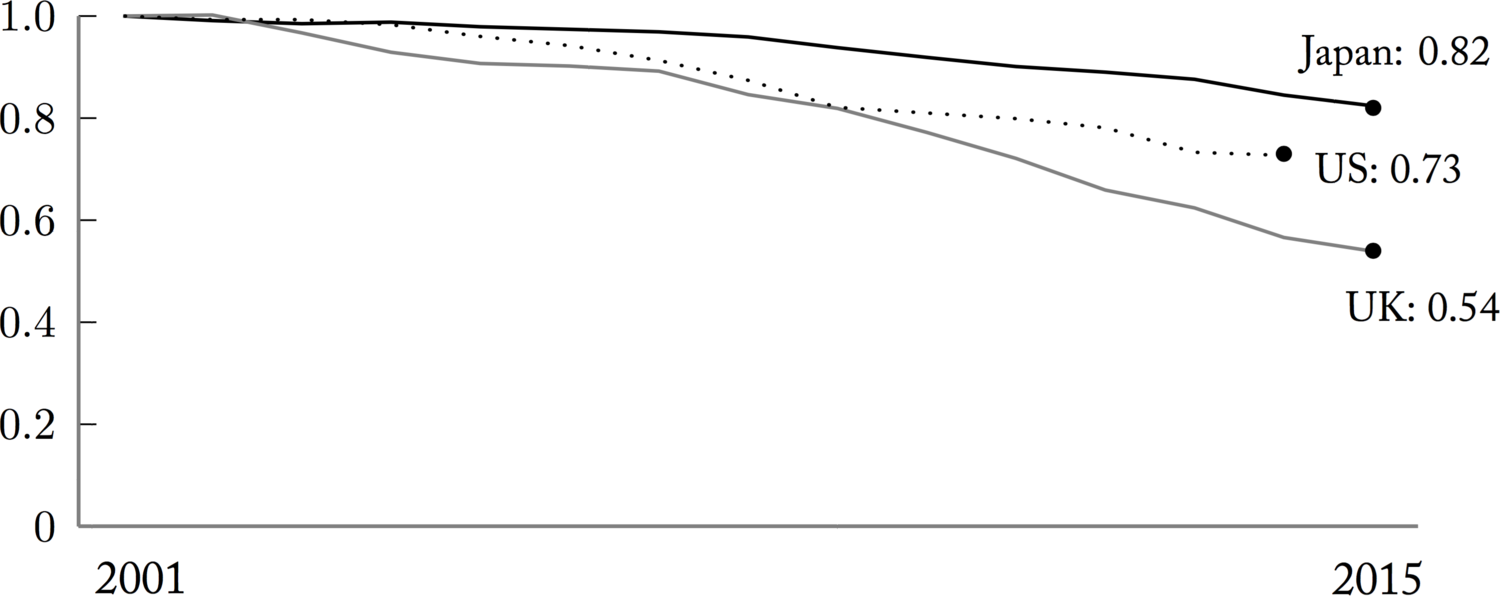
\includegraphics[height=2.08333in]{/Users/spkb/pix/circulation-2001-15-JP-US-UK.png}
\caption{Relative decline in daily national newspaper circulation in
Japan, the US and the UK, 2001-2015 (Oct 2001=1). Data Sources:
\emph{Nihon Shimbun Kyōkai} ( NSK-JNPEA ) website, UK ABCs (Guardian
Newspaper website), Newspaper Association of America (latest NAA data
available is for 2014).}
\end{figure}

The Japanese media, in the sense that it has managed to preserve itself
(as `business') in the face of competition from new media, is a success.
Why would media businesses want to change?

Another aspect worth considering is the fact that newswork is becoming
increasingly desk-bound, meaning journalists have less contact with
people outside their own organisation.(CITATIONS)

\hypertarget{references}{%
\section*{References}\label{references}}
\addcontentsline{toc}{section}{References}


\printbibliography

\end{document}
